\begin{figure}[h!]
	\centering
	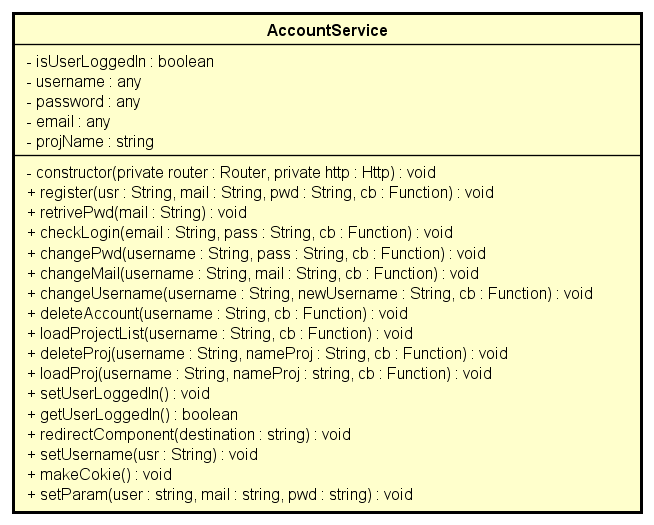
\includegraphics[scale=0.8]{res/sections/SpecificaFrontEnd/Services/Disegnetti/account.png}
	\caption{Diagramma della classe AccountService}
\end{figure}

\begin{itemize}
	\item \textbf{Descrizione:}\\
	
	\item \textbf{Utilizzo:}\\
	
	\item \textbf{Attributi:}
		\begin{itemize}
			\item \emph{-isUserLoggedIn: boolean}\\
			Serve a controllare se l'utente è autenticato
			\item \emph{-username: any}\\
			Contiene l'username dell'utente
			\item \emph{-password: any}\\
			Contiene la password dell'utente
			\item \emph{-email: any}\\
			Contiene l'email dell'utente
			\item \emph{-notOpenedProj: boolean}\\
			Controlla se il progetto è aperto o meno
			\item \emph{-projName: string}\\
			Contiene il nome del progetto attualmente aperto
		\end{itemize}
	\item \textbf{Metodi:}
		\begin{itemize}
			\item \emph{-constructor(private router: Router,private http: Http)}\\
    		Costruttore della classe\\
    		\textbf{Parametri:}
    		\begin{itemize}
    			\item \emph{router: Router}\\
    			Crea una nuova istanziazione di Router
    			\item \emph{http: Http}\\
    			Crea una nuova istanziazione di Http
    		\end{itemize}
    		\item \emph{+register(usr: String, mail: String, pwd: String, cb: Function)}\\
    		Serve per registrare un nuovo utente\\
    		\textbf{Parametri:}
    		\begin{itemize}
    			\item \emph{usr: String}\\
    			Nome utente
    			\item \emph{mail: String}\\
    			Email dell'utente
    			\item \emph{pwd: String}\\
    			Password dell'utente
    			\item \emph{cb: Function}\\
    			
    		\end{itemize}
    		\item \emph{+retrivePwd(mail: String)}\\
    		Serve per recuperare la password di un utente\\
    		\textbf{Parametri:}
    		\begin{itemize}
    			\item \emph{mail: String}\\
    			Email a cui mandare la password
    		\end{itemize}
    		\item \emph{+checkLogin(email: String, pass: String, cb: Function)}\\
    		Serve per effettuare l'autenticazione di un utente\\
    		\textbf{Parametri:}
    		\begin{itemize}
    			\item \emph{email: String}\\
    			Email dell'utente
    			\item \emph{pass: String}\\
    			Password dell'utente
    			\item \emph{cb: Function}\\
    			
    		\end{itemize}
    		\item \emph{+changePwd(username: String, pass: String, cb: Function)}\\
    		Serve per modificare la password di un utente\\
    		\textbf{Parametri:}
    		\begin{itemize}
    			\item \emph{username: String}\\
    			Nome utente
    			\item \emph{pass: String}\\
    			Password dell'utente
    			\item \emph{cb: Function}\\
    			
    		\end{itemize}
    		\item \emph{+changeMail(username: String, mail: String, cb:Function)}\\
    		Serve per modificare la mail dell'utente\\
    		\textbf{Parametri:}
    		\begin{itemize}
    			\item \emph{username: String}\\
    			Nome utente
    			\item \emph{mail: String}\\
    			Email dell'utente
    			\item \emph{String, cb:Function}\\
    			
    		\end{itemize}
    		\item \emph{+changeUsername(username: String, newUsername: String, cb: Function)}\\
    		Serve per modificare l'username dell'utente\\
    		\textbf{Parametri:}
    		\begin{itemize}
    			\item \emph{username: String}\\
    			Nome utente
    			\item \emph{newUsername: String}\\
    			Nuovo username
    			\item \emph{cb: Function}\\
    			
    		\end{itemize}
    		\item \emph{+deleteAccount(username: String, cb: Function)}\\
    		Serve per eliminare un account\\
    		\textbf{Parametri:}
    		\begin{itemize}
    			\item \emph{username: String}\\
    			Nome utente
    			\item \emph{cb: Function}\\
    			
    		\end{itemize}
    		\item \emph{+loadProjectList(username: String, cb: Function)}\\
    		Serve a caricare la lista dei progetti\\
    		\textbf{Parametri:}
    		\begin{itemize}
    			\item \emph{username: String}\\
    			Nome utente
    			\item \emph{cb: Function}\\
    			
    		\end{itemize}
    		\item \emph{+deleteProj(username: String, nameProj: String, cb: Function)}\\
    		Serve per eliminare un progetto\\
    		\textbf{Parametri:}
    		\begin{itemize}
    			\item \emph{username: String}\\
    			Nome utente
    			\item \emph{nameProj: String}\\
    			Nome del progetto
    			\item \emph{cb: Function}\\
    			
    		\end{itemize}
    		\item \emph{+loadProj(username: String, nameProj: string, cb: Function)}\\
    		Carica un progetto dalla lista progetti dell'utente\\
    		\textbf{Parametri:}
    		\begin{itemize}
    			\item \emph{username: String}\\
    			Nome utente
    			\item \emph{nameProj: string}\\
    			Nome del progetto
    			\item \emph{cb: Function}\\
    			
    		\end{itemize}
    		\item \emph{+setUserLoggedIn()}\\
    		Modifica lo stato di autenticazione dell'utente
    		\item \emph{+getUserLoggedIn()}\\
    		Ritorna true se l'utente è autenticato
    		\item \emph{+redirectComponent(destination:string)}\\
    		Questa funzione reindirizza questo componente al componente destinazione\\
    		\textbf{Parametri:}
    		\begin{itemize}
    			\item \emph{destination:string}\\
    			Componente destinazione
    		\end{itemize}
    		\item \emph{+setUsername(usr: String)}\\
    		Setta l'username dell'utente\\
    		\textbf{Parametri:}
    		\begin{itemize}
    			\item \emph{usr: String}\\
    			Nome utente
    		\end{itemize}
    		\item \emph{+makeCokie()}\\
    		Costruisce dei cookie di sessione contenenti le informazioni dell'utente
    		\item \emph{+setParam(user: string, mail:string, pwd: string)}\\
    		Setta le informazione in AccountService\\
    		\textbf{Parametri:}
    		\begin{itemize}
    			\item \emph{user: string}\\
    			Nome utente
    			\item \emph{mail:string}\\
    			Email dell'utente
    			\item \emph{pwd: string}\\
    			Password dell'utente
    		\end{itemize}
    		\item \emph{+logout()}\\
    		Esegue il logout
		\end{itemize}
\end{itemize}